\section*{Questões}
\paragraph{1.}

\subparagraph{a.}
Capture do primeiro ICMP \emph{Echo Request} enviado em ambas as interfaces:

\begin{figure}[h]
\centering
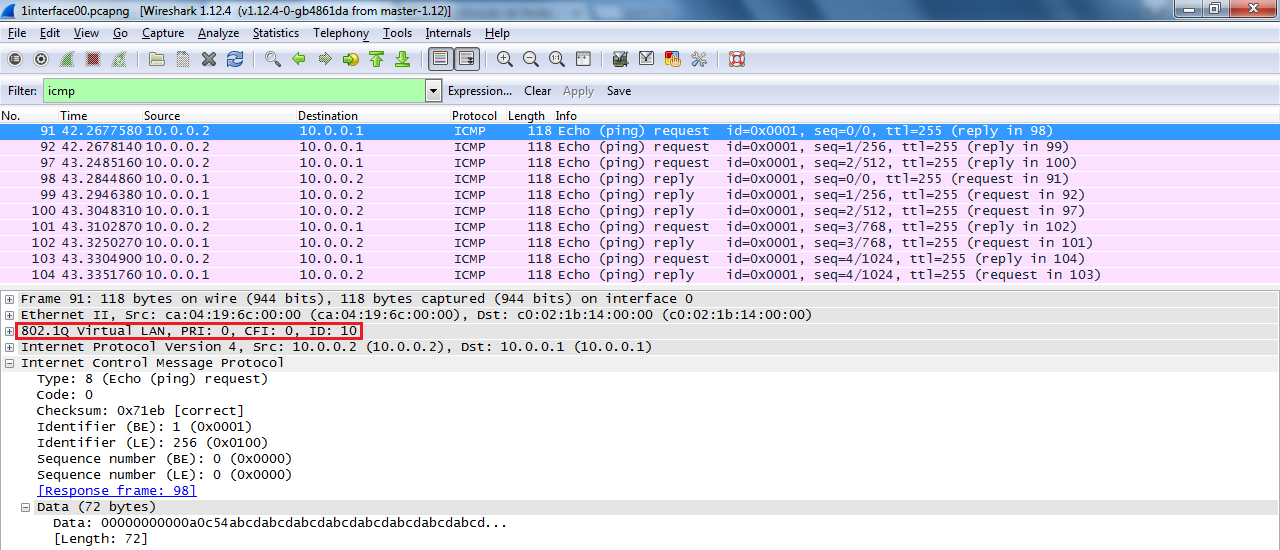
\includegraphics[width=1\textwidth, height=0.33\textheight]{1_interface00-groucho.png}
\label{fig:2-capturaWireshark}
\caption{Captura \emph{wireshark} na interface \textsf{f0/0} de \textsf{groucho}.}
\end{figure}

\begin{figure}[h]
\centering
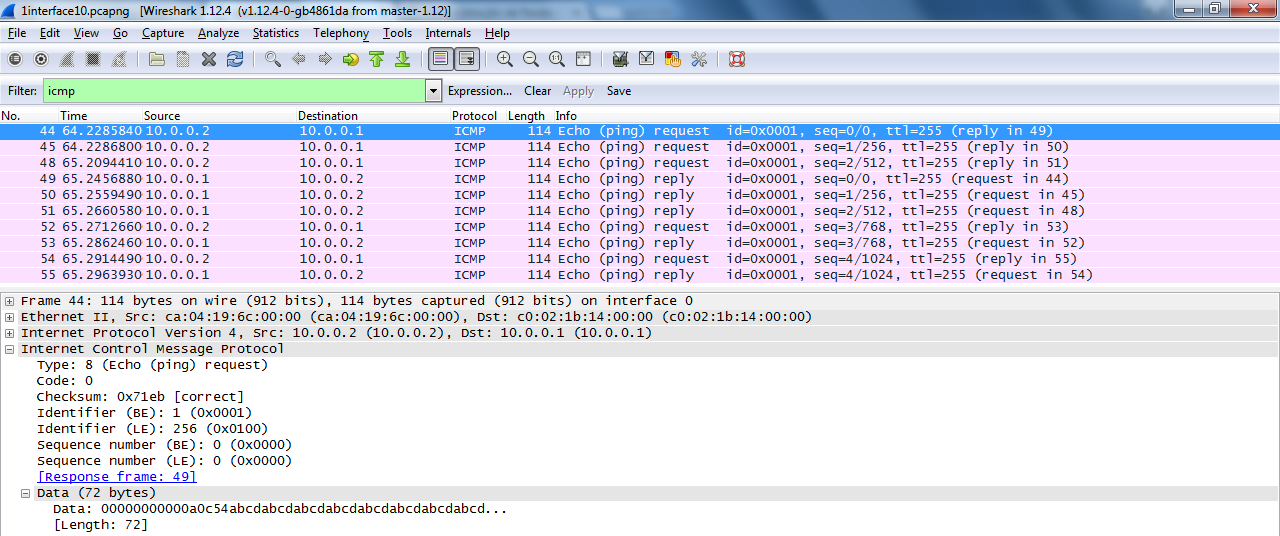
\includegraphics[width=1\textwidth, height=0.33\textheight]{1_interface10-R1.png}
\label{fig:2-capturaWireshark}
\caption{Captura \emph{wireshark} na interface \textsf{f1/0} de \textsf{R1}.}
\end{figure}


\subparagraph{b.}
Quais foram as diferenças encontradas e a que se devem? (texRes)


\paragraph{2.}
Altere o endereço IP de averell para 10.0.0.4, que pertence à mesma subnet de groucho. Faça um ping de averell para groucho. Diga o que observa e explique a razão para ser assim.


\paragraph{3.}
 Faça um ping de groucho para averell. O que observa em relação aos pacotes ICMP? (capRes + texRes)
 
\begin{figure}[h]
\centering
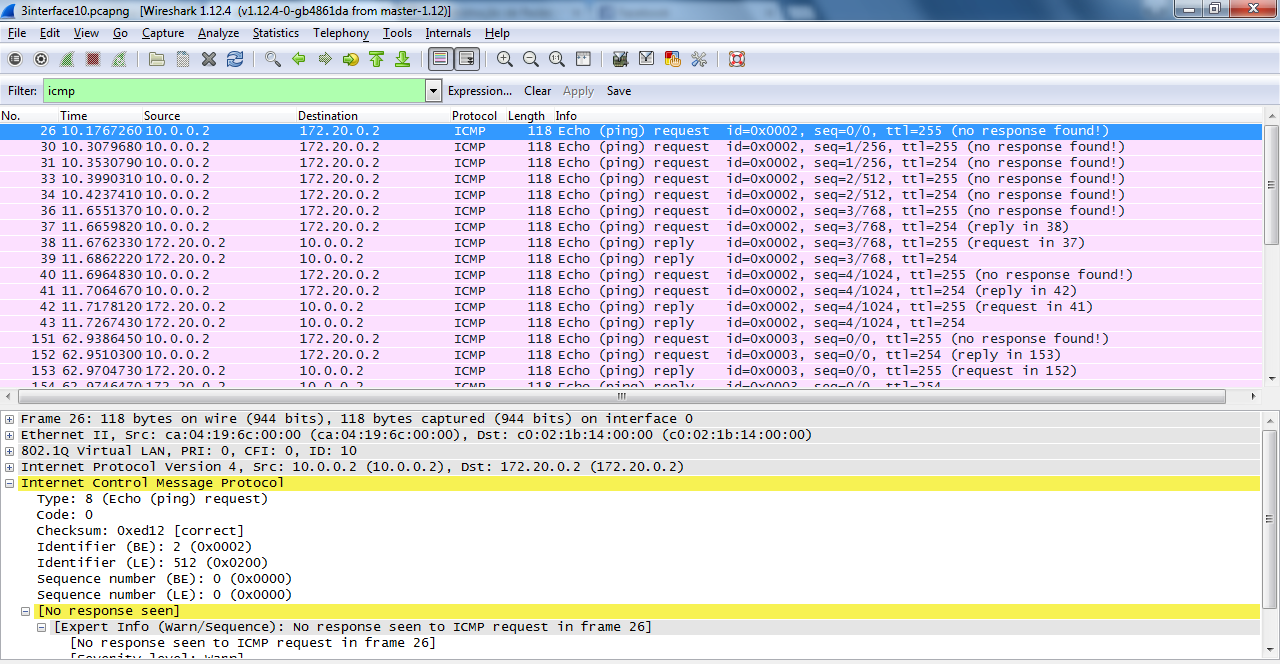
\includegraphics[width=1\textwidth, height=0.33\textheight]{3_interface10_R1.png}
\label{fig:2-capturaWireshark}
\caption{Captura \emph{wireshark} na interface \textsf{f1/0} de \textsf{R1}.}
\end{figure}


\paragraph{4.}

\subparagraph{a.}
Para que a ligação entre \textsf{R1} e o terminal \textsf{linux} funcionar em modo \emph{trunk} tivemos de realizar as seguintes configurações.

No \emph{router} \textsf{R1}:
\begin{verbatim}
interface FastEthernet 1/3
switchport trunk encapsulation dot1q
switchport mode trunk
\end{verbatim}

No \textsf{linux}:
\begin{verbatim}
[root@Labs5610 ar]# modprobe 8021q
[root@Labs5610 ar]# vconfig add tap0 10
Added VLAN with VID == 10 to IF -:tap0:-
[root@Labs5610 ar]# 
[root@Labs5610 ar]# ifconfig tap0.10 10.0.0.5 netmask 255.255.255.0 up
\end{verbatim}


\subparagraph{b.}
Capture de um pacote do ping (ICMP) enviado em ambas as interfaces:

\begin{figure}[h]
\centering
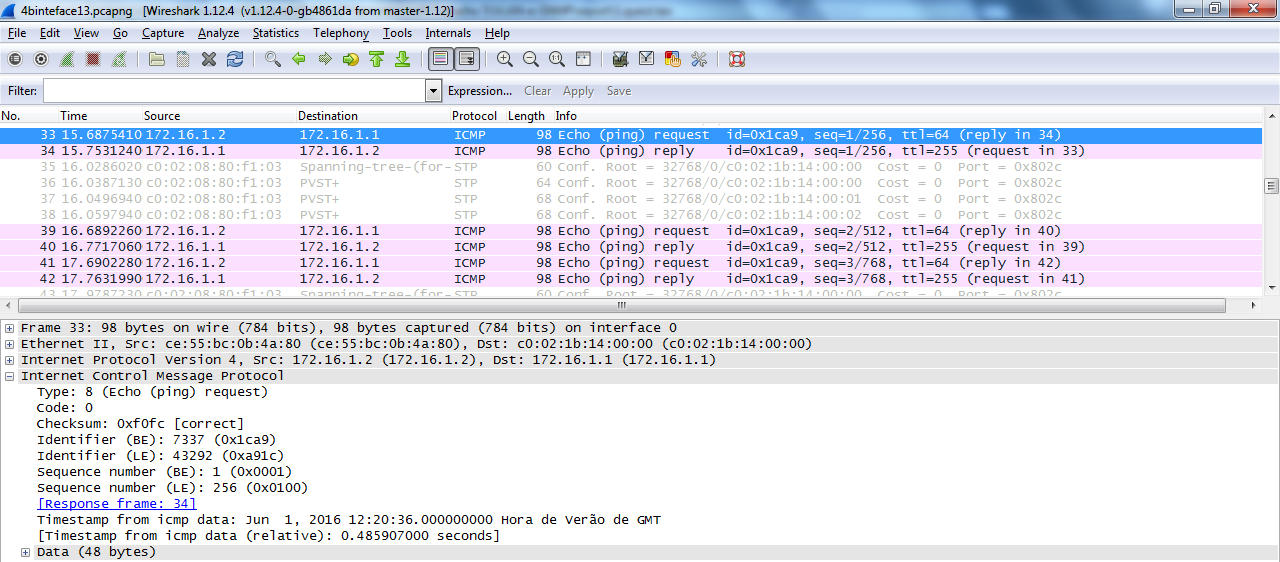
\includegraphics[width=1\textwidth, height=0.33\textheight]{ping_VLAN1.png}
\label{fig:2-capturaWireshark}
\caption{Captura \emph{wireshark} de um pacote do \texttt{ping} enviado do terminal \textsf{linux} para a \textsf{VLAN 1}.}
\end{figure}

\begin{figure}[h]
\centering
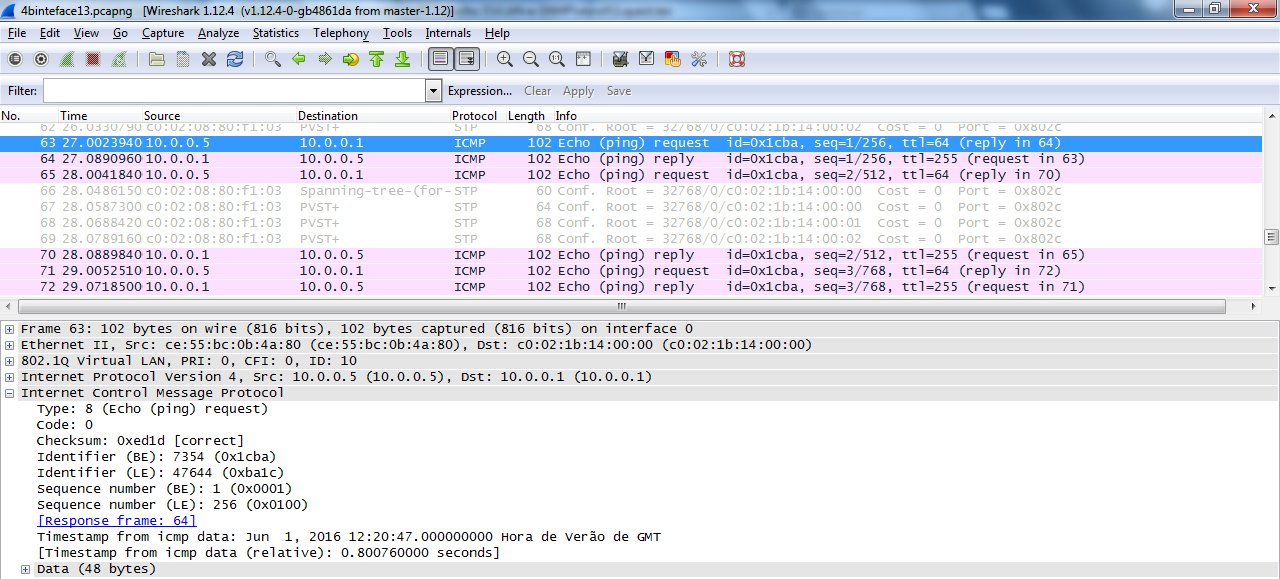
\includegraphics[width=1\textwidth, height=0.33\textheight]{ping_VLAN10.png}
\label{fig:2-capturaWireshark}
\caption{Captura \emph{wireshark} de um pacote do \texttt{ping} enviado do terminal \textsf{linux} para a \textsf{VLAN 10}.}
\end{figure}


\subparagraph{c.}
Como explica o que observou na alínea anterior? (texRes)


\paragraph{5.}

\subparagraph{a.}
Tente fazer um get ao OID iso.org.dod.internet.mgmt.mib-2.system.sysDescr de R1. Por que razão não conseguiu? (texRes)

\begin{verbatim}
[root@Labs5610 ar]# snmpget -v 2c -c Leitura 172.16.1.1 iso.org.dod.internet.mgmt.mib-2.system.sysDescr
SNMPv2-MIB::sysDescr = No Such Instance currently exists at this OID
\end{verbatim}

"When we want to actually use this OID in practice, we’ll need to tack on another number to get the value of this variable. That is, we will need to append a .0, representing the first (and only, since a device cannot have more than one description) instance of this object.
"


\subparagraph{b.}
\begin{verbatim}
[root@Labs5610 ar]# snmpget -v 2c -c Leitura 172.16.1.1 iso.org.dod.internet.mgmt.mib-2.system.sysDescr.0
SNMPv2-MIB::sysDescr.0 = STRING: Cisco IOS Software, 2600 Software (C2691-ADVIPSERVICESK9-M), Version 12.4(15)T6, RELEASE SOFTWARE (fc2)
Technical Support: http://www.cisco.com/techsupport
Copyright (c) 1986-2008 by Cisco Systems, Inc.
Compiled Mon 07-Jul-08 04:30 by prod_rel_team
\end{verbatim}


\subparagraph{c.}
Faça um getnext ao mesmo OID usado na alínea anterior. Para que serve o getnext? (texRes)

\begin{verbatim}
[root@Labs5610 ar]# snmpgetnext -v 2c -c Leitura 172.16.1.1 iso.org.dod.internet.mgmt.mib-2.system.sysDescr.0
SNMPv2-MIB::sysObjectID.0 = OID: SNMPv2-SMI::enterprises.9.1.122
\end{verbatim}


\subparagraph{d.}
Diga para que serve o walk e explique como funciona, indicando as mensagens SNMP a partir das quais se constrói e as condições de terminação. (capRes + texRes)

\begin{figure}[h]
\centering
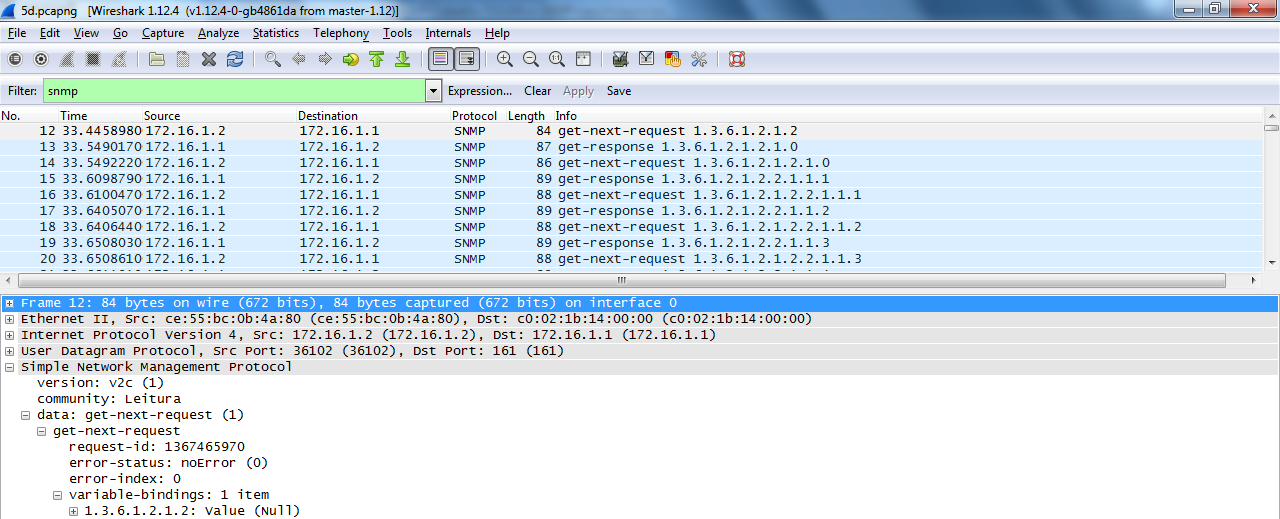
\includegraphics[width=1\textwidth, height=0.33\textheight]{5d.png}
\label{fig:2-capturaWireshark}
\caption{Captura \emph{wireshark} de pacotes SNMP na interface \textsf{f1/3} de \textsf{R1}.}
\end{figure}


\subparagraph{e.}
Com base nos resultados da alínea anterior, diga quantas interfaces tem o router e quais são elas. (texRes)


\subparagraph{f.}
Resultado do \texttt{get}:
\begin{verbatim}
[root@Labs5610 ar]# snmpget -v 2c -c Leitura 172.16.1.1 iso.org.dod.internet.mgmt.mib-2.system.sysName.0
SNMPv2-MIB::sysName.0 = STRING: R1
\end{verbatim}

Comando usado para fazer o \texttt{set}:
\begin{verbatim}
[root@Labs5610 ar]# snmpset -v 2c -c Escrita 172.16.1.1 iso.org.dod.internet.mgmt.mib-2.system.sysName.0 s R2
SNMPv2-MIB::sysName.0 = STRING: R2
\end{verbatim}


\subparagraph{g.}
Faça um walk e um bulkwalk à sub-árvore system da MIB-2. Qual é a diferença entre estes dois comandos e em que se traduz na prática? (2×capRes + texRes)

\begin{figure}[h]
\centering
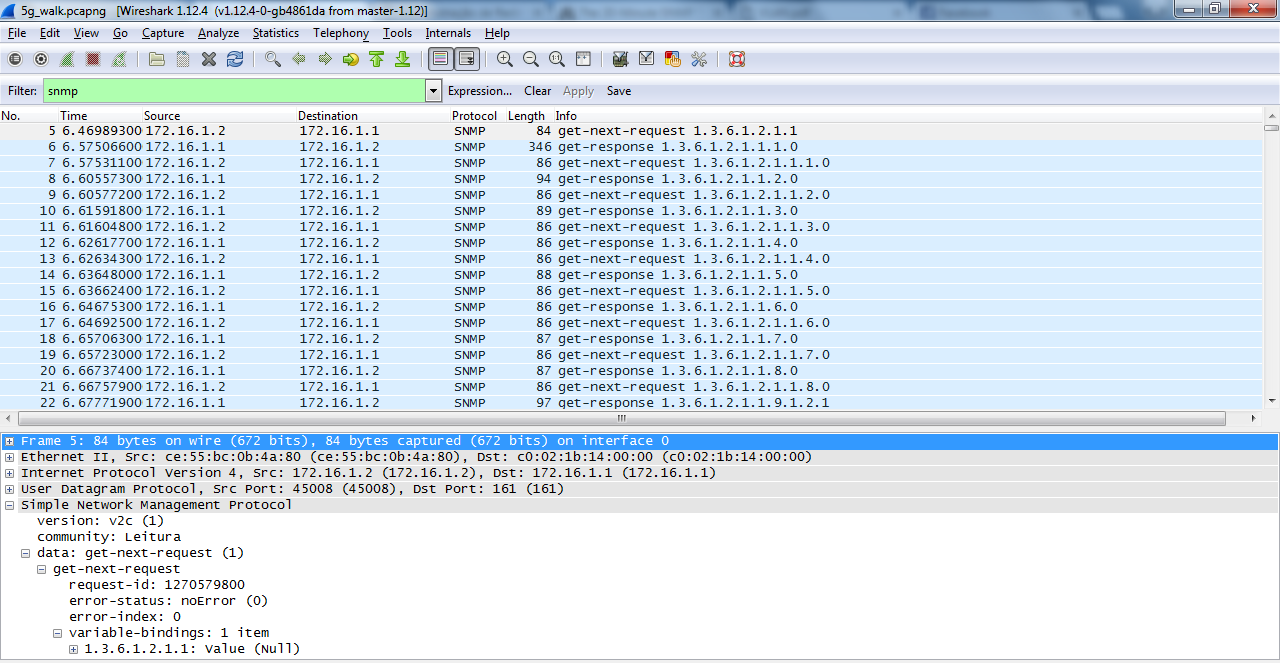
\includegraphics[width=1\textwidth, height=0.33\textheight]{5g_walk.png}
\label{fig:2-capturaWireshark}
\caption{Captura \emph{wireshark} de pacotes \texttt{snmpwalk}.}
\end{figure}

\begin{figure}[h]
\centering
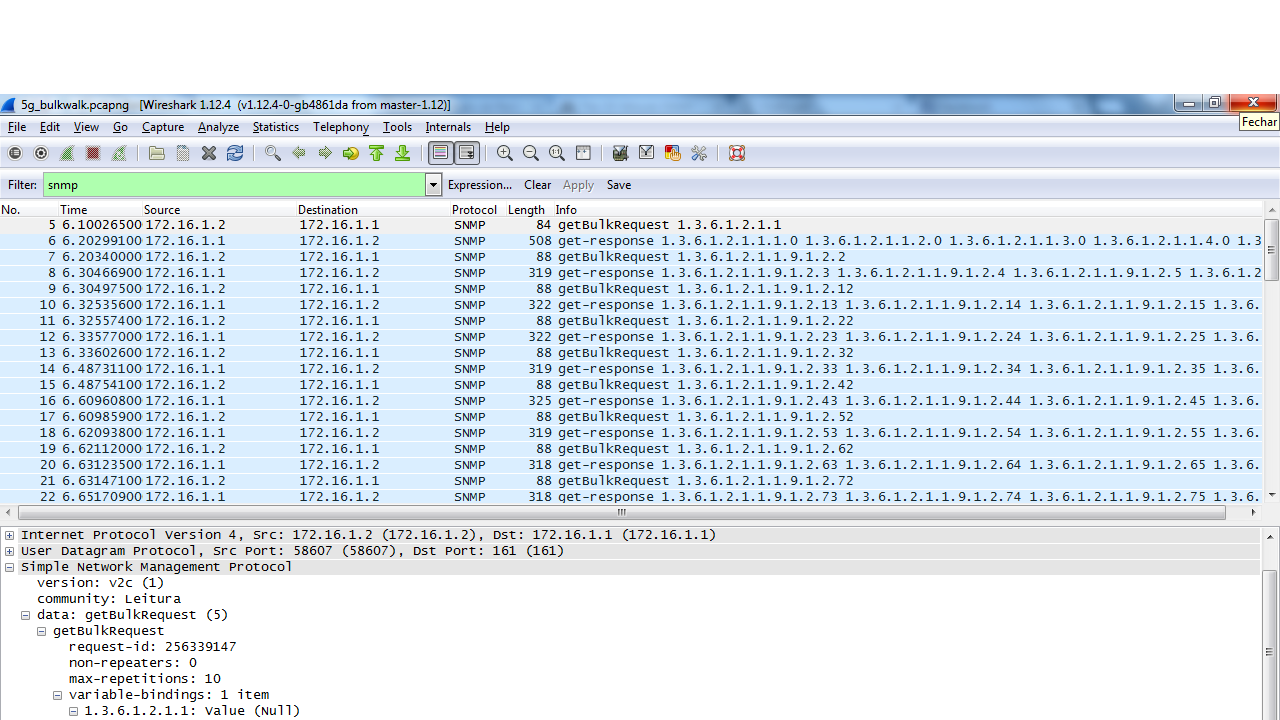
\includegraphics[width=1\textwidth, height=0.33\textheight]{5g_bulkwalk.png}
\label{fig:2-capturaWireshark}
\caption{Captura \emph{wireshark} de pacotes \texttt{bulkwalk}.}
\end{figure}


\subparagraph{h.}
Informação sobre as interfaces de \textsf{R1}:
\begin{verbatim}
[root@Labs5610 ar]# snmpnetstat -v 2c -Ci -c Leitura 172.16.1.1
Name      Mtu Network     Address    Ipkts Ierrs Opkts Oerrs Queue
Fa0/0    1500                            0     0     0     0     0
Fa0/1    1500                            0     0     0     0     0
Fa1/0    1500                            0     0     0     0     0
Fa1/1    1500                            0     0     0     0     0
Fa1/2    1500                            0     0     0     0     0
Fa1/3    1500                            0     0     0     0     0
Fa1/4    1500                            0     0     0     0     0
Fa1/5    1500                            0     0     0     0     0
Fa1/6    1500                            0     0     0     0     0
Fa1/7    1500                            0     0     0     0     0
Fa1/8    1500                            0     0     0     0     0
Fa1/9    1500                            0     0     0     0     0
Fa1/10   1500                            0     0     0     0     0
Fa1/11   1500                            0     0     0     0     0
Fa1/12   1500                            0     0     0     0     0
Fa1/13   1500                            0     0     0     0     0
Fa1/14   1500                            0     0     0     0     0
Fa1/15   1500                            0     0     0     0     0
Nu0      1500                            0     0     0     0     0
Vl1      1500 172.16.1/24 172.16.1.1  1178     0  1183     0     0
Vl10     1500 10.0.0/24   10.0.0.1      61     0    39     0     0
Vl20     1500 172.20.0/24 172.20.0.1    47     0    29     0     0
\end{verbatim}

Informação sobre a tabela de encaminhamento de \textsf{R1}:
\begin{verbatim}
[root@Labs5610 ar]# snmpnetstat -v 2c -Cr -c Leitura 172.16.1.1
Routing tables (ipCidrRouteTable)
Destination                Gateway            Flags   Interface
10.0.0/24                  *                  <U>     Vl10
172.16.1/24                *                  <U>     Vl1
172.20.0/24                *                  <U>     Vl20
\end{verbatim}


\paragraph{6.}

\subparagraph{a.}
Tabela de informação sobre os endereços IP de \textsf{R1}:
\begin{verbatim}
[root@Labs5610 ar]# snmptable -v 2c -c Leitura 172.16.1.1 ip.ipAddrTable
SNMP table: IP-MIB::ipAddrTable

 ipAdEntAddr ipAdEntIfIndex ipAdEntNetMask ipAdEntBcastAddr ipAdEntReasmMaxSize
    10.0.0.1             22  255.255.255.0                1               18024
  172.16.1.1             21  255.255.255.0                1               18024
  172.20.0.1             23  255.255.255.0                1               18024

\end{verbatim}


\subparagraph{b.}
Com base na sua definição no módulo IP-MIB, explique o que faz com que ip.ipAddrTable seja uma tabela. (texRes)


\subparagraph{c.}
Diga como se mapeiam as linhas (índices) e as colunas de uma tabela em OIDs na estrutura em árvore da MIB. (texRes)


\paragraph{7.}

\subparagraph{a.}
Inicie uma nova captura wireshark na interface f1/3 de R1. Simule a falha da ligação da interface f1/2 desactivando-a administrativamente (shutdown). O que observa? (capRes + texRes)

\begin{figure}[h]
\centering
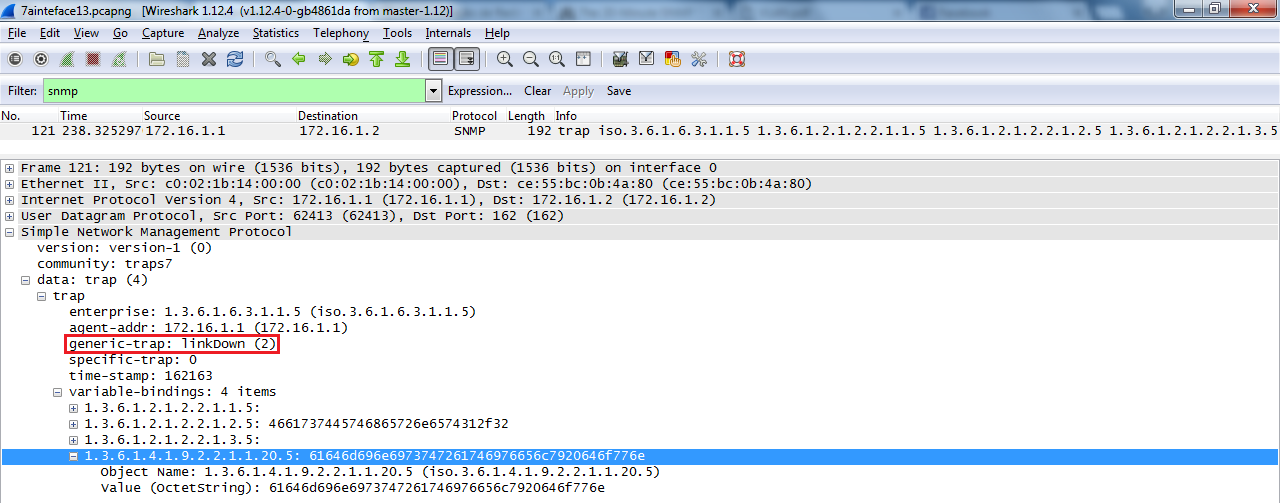
\includegraphics[width=1\textwidth, height=0.33\textheight]{7a.png}
\label{fig:2-capturaWireshark}
\caption{Captura \emph{wireshark} na interface \textsf{1/3} de \textsf{R1}.}
\end{figure}


\subparagraph{b.}
Captura de pacotes SNMP na interface \textsf{f1/3} de \textsf{R1}:

\begin{figure}[h]
\centering
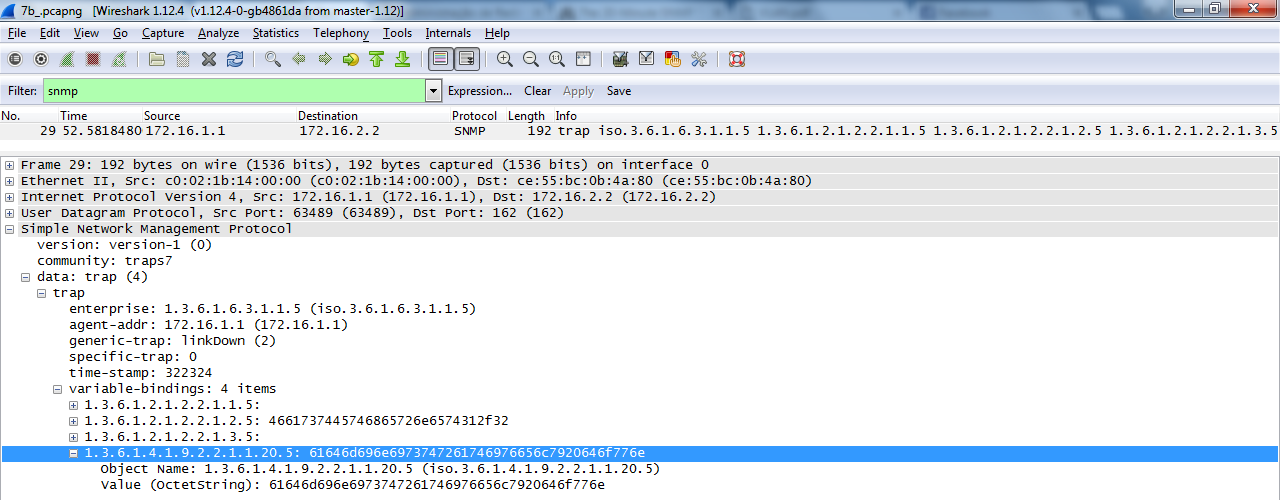
\includegraphics[width=1\textwidth, height=0.33\textheight]{7b.png}
\label{fig:2-capturaWireshark}
\caption{Captura \emph{wireshark} na interface \textsf{1/3} de \textsf{R1}.}
\end{figure}


\subparagraph{c.}
Captura de pacotes SNMP na interface \textsf{f1/3} de \textsf{R1}:

\begin{figure}[h]
\centering
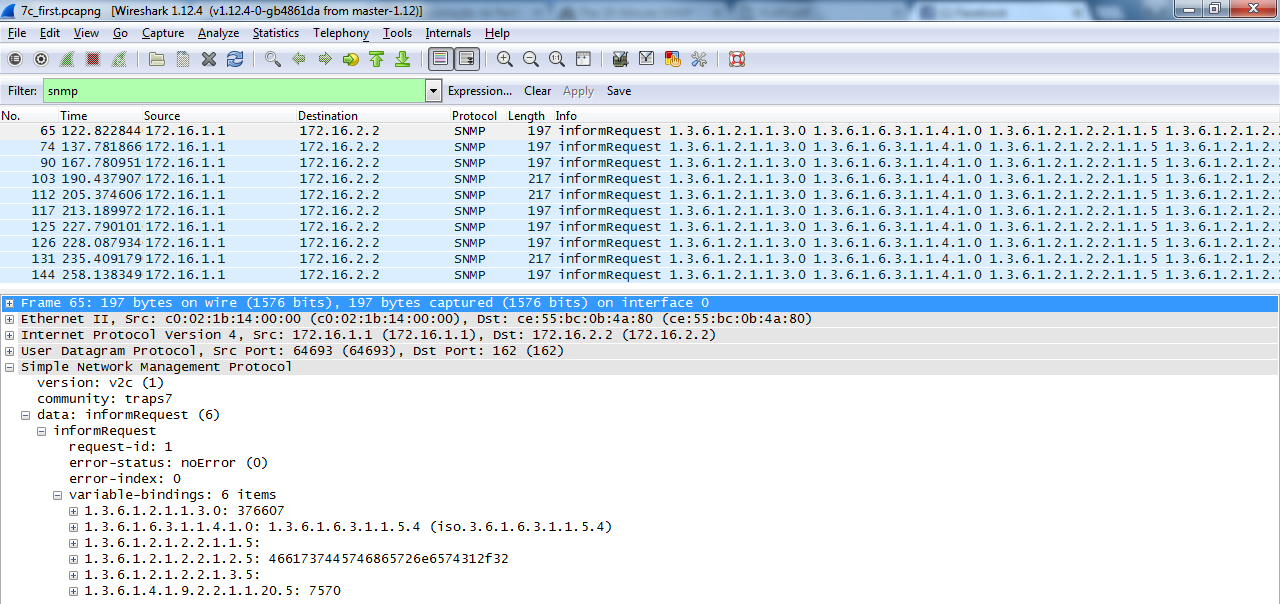
\includegraphics[width=1\textwidth, height=0.33\textheight]{7c.png}
\label{fig:2-capturaWireshark}
\caption{Captura \emph{wireshark} na interface \textsf{1/3} de \textsf{R1}.}
\end{figure}


\subparagraph{d.}
Captura de pacotes SNMP na interface \textsf{f1/3} de \textsf{R1}:

\begin{figure}[h]
\centering
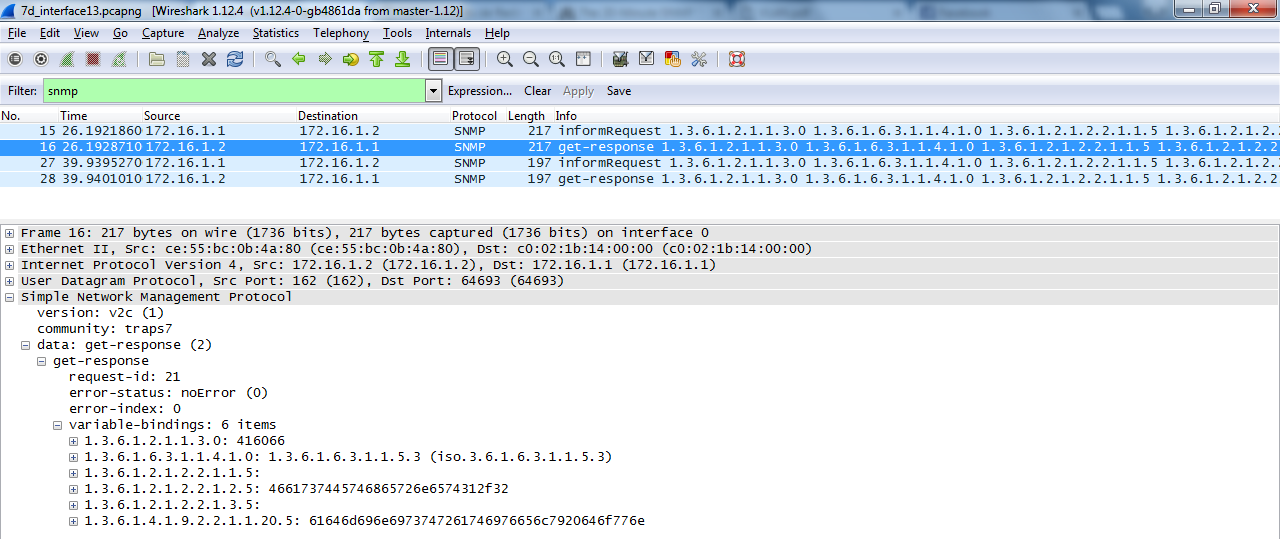
\includegraphics[width=1\textwidth, height=0.33\textheight]{7d.png}
\label{fig:2-capturaWireshark}
\caption{Captura \emph{wireshark} na interface \textsf{1/3} de \textsf{R1}.}
\end{figure}


\subparagraph{e.}
Com base nas alíneas anteriores, comente as diferenças entre o uso de informs e de traps, bem como as implicações práticas dessas diferenças. (texRes)


\paragraph{8.}

\subparagraph{a.}
Captura dos pacotes trocados quando executados os seguintes comandos:

\begin{itemize}
\item \texttt{snmpgetnext -v2c -c Leitura 172.16.1.1 system.sysName}:

\begin{figure}[h]
\centering
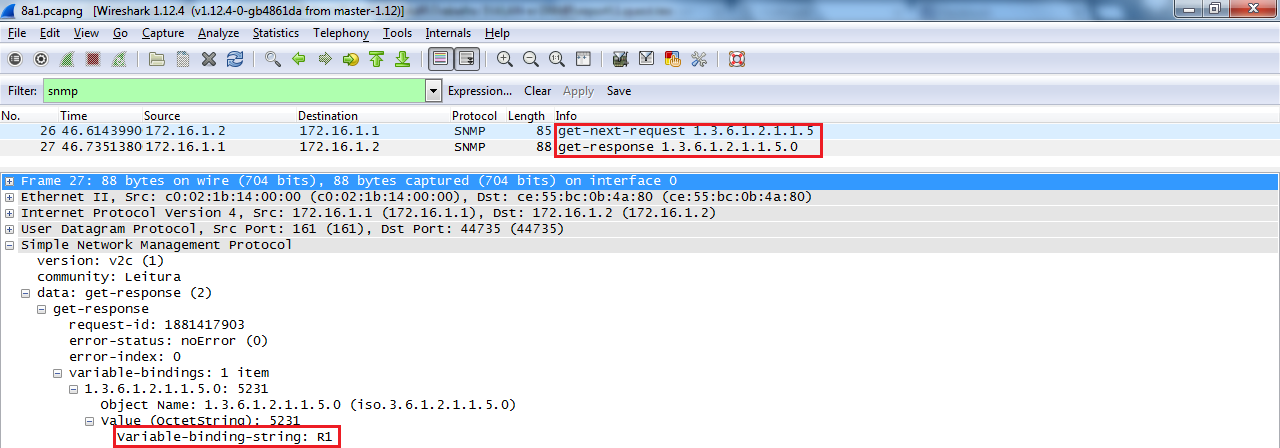
\includegraphics[width=1\textwidth, height=0.33\textheight]{8a1.png}
\label{fig:2-capturaWireshark}
\caption{Captura \emph{wireshark} na interface \textsf{1/3} de \textsf{R1}.}
\end{figure}


\item \texttt{snmpgetnext -v3 -l authNoPriv -u grupo11 -a md5 -A passlimi 172.16.1.1 system.sysName}:

\begin{figure}[h]
\centering
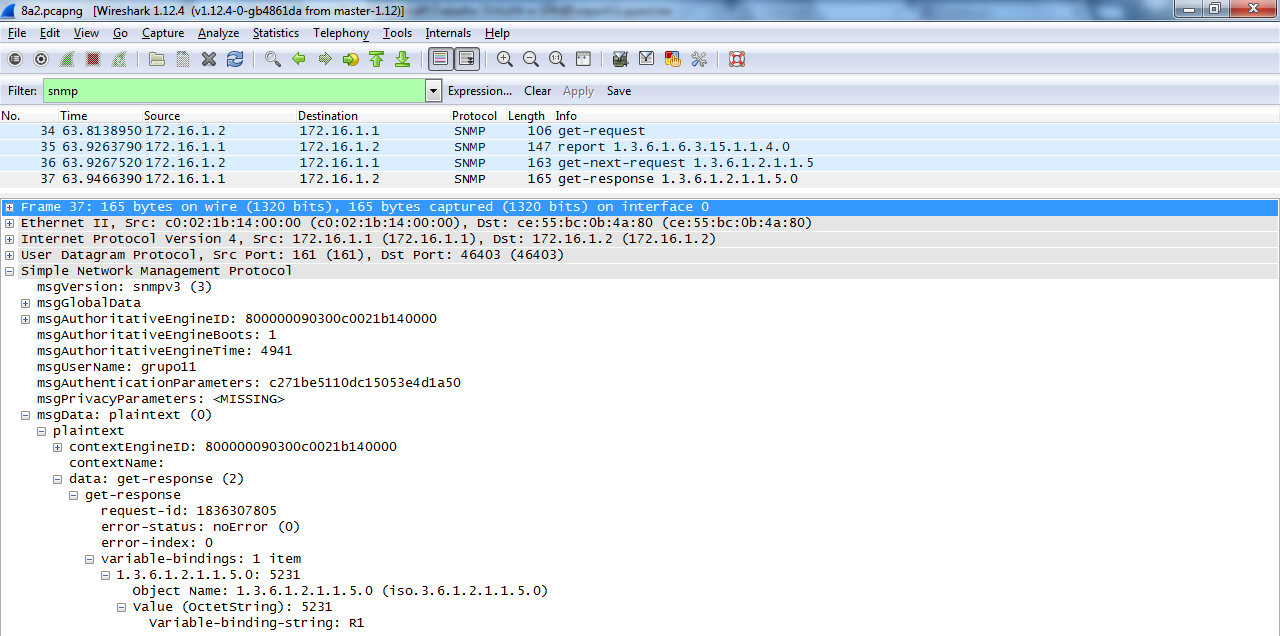
\includegraphics[width=1\textwidth, height=0.33\textheight]{8a2.png}
\label{fig:2-capturaWireshark}
\caption{Captura \emph{wireshark} na interface \textsf{1/3} de \textsf{R1}.}
\end{figure}


\item \texttt{snmpgetnext -v3 -l authPriv -u cifragrupo11 -a md5 -A passlimi -x des -X cifralimi 172.16.1.1 system.sysName}:

\begin{figure}[h]
\centering
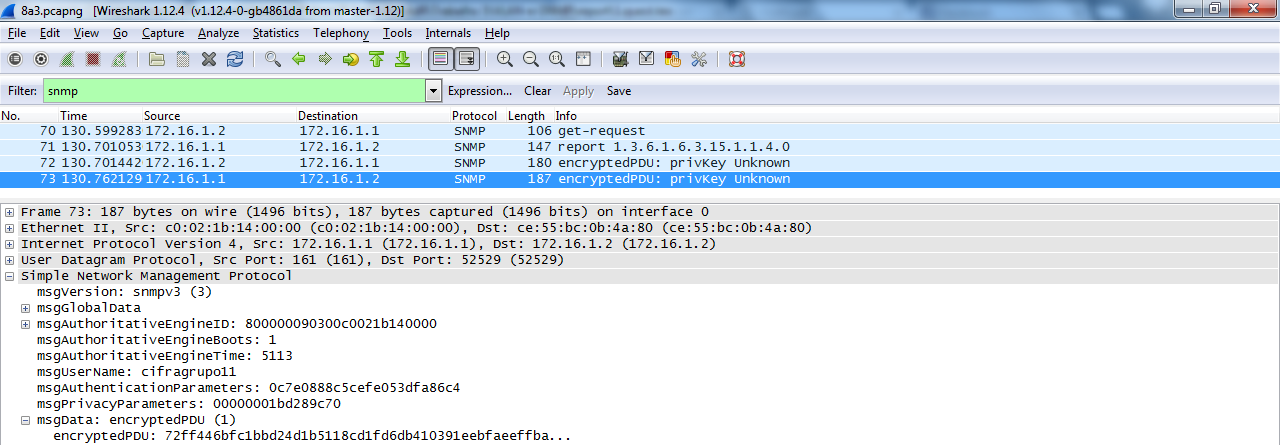
\includegraphics[width=1\textwidth, height=0.33\textheight]{8a3.png}
\label{fig:2-capturaWireshark}
\caption{Captura \emph{wireshark} na interface \textsf{1/3} de \textsf{R1}.}
\end{figure}

\end{itemize}


\subparagraph{b.}
Compare a segurança nos três casos. (texRes)